\documentclass{article}

% If you're new to LaTeX, here's some short tutorials:
% https://www.overleaf.com/learn/latex/Learn_LaTeX_in_30_minutes
% https://en.wikibooks.org/wiki/LaTeX/Basics

% Formatting
\usepackage{subfig}
\usepackage{hyperref}
\usepackage{subcaption}
\usepackage[utf8]{inputenc}
\usepackage[margin=1in]{geometry}
\usepackage[titletoc,title]{appendix}

% Math
% https://www.overleaf.com/learn/latex/Mathematical_expressions
% https://en.wikibooks.org/wiki/LaTeX/Mathematics
\usepackage{amsmath,amsfonts,amssymb,mathtools}

% Images
% https://www.overleaf.com/learn/latex/Inserting_Images
% https://en.wikibooks.org/wiki/LaTeX/Floats,_Figures_and_Captions
\usepackage{graphicx,float}

% Tables
% https://www.overleaf.com/learn/latex/Tables
% https://en.wikibooks.org/wiki/LaTeX/Tables

% Algorithms
% https://www.overleaf.com/learn/latex/algorithms
% https://en.wikibooks.org/wiki/LaTeX/Algorithms
\usepackage[ruled,vlined]{algorithm2e}
\usepackage{algorithmic}

% Code syntax highlighting
% https://www.overleaf.com/learn/latex/Code_Highlighting_with_minted
\usepackage{minted}
\usemintedstyle{borland}

% References
% https://www.overleaf.com/learn/latex/Bibliography_management_in_LaTeX
% https://en.wikibooks.org/wiki/LaTeX/Bibliography_Management
\usepackage{biblatex}
\addbibresource{references.bib}

% Title content
\title{
    \textbf{CSE343: Machine Learning} \\ \vspace*{-5pt}
    \textbf{\large{Assignment-2}}
}

\author{\href{mailto:shubham21099@iiitd.ac.in}{Shubham Sharma (2021099)}}
\date{\today}

\geometry{a4paper, left=20mm, right=20mm, top=20mm, bottom=20mm}

\begin{document}

\maketitle

% Abstract
% \begin{abstract}
%     Add your abstract here.
% \end{abstract}

% Introduction and Overview
\section{Section A (Theoretical)}
% Add your introduction and overview here.

% Example Subsection
\subsection*{Solution (a)}
\subsubsection*{Given Values}

\begin{itemize}
    \item $P(D) = 0.8$: Probability of issuing a dividend.
    \item $P(ND) = 0.2$: Probability of not issuing a dividend.
    \item Profit increase for dividend-issuing companies $\sim \mathcal{N}(10\%, 36\%)$.
    \item Profit increase for non-dividend-issuing companies $\sim \mathcal{N}(0\%, 36\%)$.
    \item Observed profit increase: $P = 4\%$.
\end{itemize}

\hspace{-20pt}
We want to calculate $P(D | P)$, the probability of issuing a dividend given a 4\% profit increase. By Bayes' Theorem:

\[
P(D | P) = \frac{P(P | D) P(D)}{P(P | D) P(D) + P(P | ND) P(ND)}
\]

\subsubsection*{Step 1: Likelihood of Profit Increase}

Both the dividend and non-dividend cases follow normal distributions; we can use the normal distribution to calculate the likelihoods.

\[
P(P | D) = \frac{1}{\sqrt{2\pi\sigma^2}} e^{-\frac{(4 - 10)^2}{2\sigma^2}}
\]

\[
P(P | ND) = \frac{1}{\sqrt{2\pi\sigma^2}} e^{-\frac{(4 - 0)^2}{2\sigma^2}}
\]

\hspace{-17pt}
Since the standard deviation is the same for both, the normalization constant cancels out, so we only need to calculate the exponentials.

\vspace{3pt}
For $P(P | D)$:
\[
P(P | D) = e^{-\frac{(4 - 10)^2}{2 \times 36^2}} = e^{-0.01389} \approx 0.9862
\]

For $P(P | ND)$:
\[
P(P | ND) = e^{-\frac{(4 - 0)^2}{2 \times 36^2}} = e^{-0.00617} \approx 0.9938
\]

\subsubsection*{Step 2: Apply Bayes' Theorem}

Substitute the values into Bayes' Theorem:

\[
P(D | P) = \frac{0.9862 \times 0.8}{0.9862 \times 0.8 + 0.9938 \times 0.2} = \frac{0.78896}{0.78896 + 0.19876} = \frac{0.78896}{0.98772} \approx 0.798
\]

\vspace{10pt}
\hspace{-17pt}
The likelihood that a company with a 4\% profit increase will issue a dividend is approximately $\mathbf{79\%}$.


\vspace{10pt}
\subsection*{Solution (b)}
\begin{table}[H]
    \centering
    \begin{tabular}{|l|c|c|c|c|}
        \hline
        \textbf{Class Time} & \textbf{Had Proper Sleep} & \textbf{Weather} & \textbf{Attended ML Class} \\ \hline
        Morning & YES & COOL & YES \\ \hline
        Morning & NO & RAINY & NO \\ \hline
        Morning & NO & COOL & YES \\ \hline
        Morning & YES & HOT & YES \\ \hline
        Noon & YES & COOL & YES \\ \hline
        Noon & NO & HOT & NO \\ \hline
        Noon & NO & COOL & NO \\ \hline
        Noon & YES & HOT & YES \\ \hline
        Afternoon & YES & COOL & YES \\ \hline
        Afternoon & NO & RAINY & NO \\ \hline
        Afternoon & NO & HOT & NO \\ \hline
        Afternoon & YES & HOT & YES \\ \hline
    \end{tabular}
    \caption{Given Dataset}
\end{table}

\subsection*{Step 1: Calculating the Entropy of the Entire Dataset}
\begin{itemize}
    \item Total `Yes' for attending the ML class: 7
    \item Total `No' for attending the ML class: 5
    \item Total instances: 12
\end{itemize}

\[
\text{Entropy}(S) = - \sum_{i=1}^{c} p_i \log_2(p_i)
\]

The entropy of the entire dataset is:

\[
\text{Entropy}(S) = -\frac{7}{12} \log_2\left(\frac{7}{12}\right) - \frac{5}{12} \log_2\left(\frac{5}{12}\right) = 0.98
\]

\subsection*{Step 2: Information Gain of Each Feature}

\textbf{1. Class Time}

Feature \textbf{Class Time} has three attributes: Morning, Noon, and Afternoon
\begin{itemize}
    \item Entropy for Morning: 
    \[
    \text{Entropy}(S_{\text{Morning}}) = -\frac{3}{4} \log_2\left(\frac{3}{4}\right) - \frac{1}{4} \log_2\left(\frac{1}{4}\right) = 0.811
    \]
    \item Entropy for Noon: 
    \[
    \text{Entropy}(S_{\text{Noon}}) = -\frac{2}{4} \log_2\left(\frac{2}{4}\right) - \frac{2}{4} \log_2\left(\frac{2}{4}\right) = 1
    \]
    \item Entropy for Afternoon: 
    \[
    \text{Entropy}(S_{\text{Afternoon}}) = -\frac{2}{4} \log_2\left(\frac{2}{4}\right) - \frac{2}{4} \log_2\left(\frac{2}{4}\right) = 1
    \]
\end{itemize}

Now, the Information Gain for Class Time is:

\[
\text{IG}(\text{Class Time}) = 0.957 - \frac{4}{12}(0.811) - \frac{4}{12}(1) - \frac{4}{12}(1) = \textbf{0.04}
\]

\hspace{-20pt}
\textbf{2. Proper Sleep}

Feature \textbf{Proper Sleep} has two attributes: Yes and No

\begin{itemize}
    \item Entropy for Proper Sleep = Yes:
    \[
    \text{Entropy}(S_{\text{Yes}}) = -\frac{6}{6} \log_2\left(\frac{6}{6}\right) = 0
    \]
    \item Entropy for Proper Sleep = No:
    \[
    \text{Entropy}(S_{\text{No}}) = -\frac{1}{6} \log_2\left(\frac{1}{6}\right) - \frac{5}{6} \log_2\left(\frac{5}{6}\right) = 0.65
    \]
\end{itemize}

Now, the Information Gain for Proper Sleep is:

\[
\text{IG}(\text{Proper Sleep}) = 0.957 - \frac{6}{12}(0) - \frac{6}{12}(0.65) = \textbf{0.655}
\]

\hspace{-20pt}
\textbf{3. Weather}

Feature \textbf{Weather} has three attributes: Hot, Cool, and Rainy

\begin{itemize}
    \item Entropy for Hot:
    \[
    \text{Entropy}(S_{\text{Hot}}) = -\frac{3}{5} \log_2\left(\frac{3}{5}\right) - \frac{2}{5} \log_2\left(\frac{2}{5}\right) = 0.97
    \]
    \item Entropy for Cool:
    \[
    \text{Entropy}(S_{\text{Cool}}) = -\frac{4}{5} \log_2\left(\frac{4}{5}\right) - \frac{1}{5} \log_2\left(\frac{1}{5}\right) = 0.72
    \]
    \item Entropy for Rainy:
    \[
    \text{Entropy}(S_{\text{Rainy}}) = 0
    \]
\end{itemize}

Now, the Information Gain for Weather is:

\[
\text{IG}(\text{Weather}) = 0.957 - \frac{5}{12}(0.97) - \frac{5}{12}(0.72) - \frac{2}{12}(0) = \textbf{0.27}
\]

\subsection*{Step 3: Choosing the Root Node}

Among all attributes, the attribute Proper Sleep has the \textbf{highest} Information Gain (\textbf{0.632}). Hence, Proper Sleep is selected as the \textbf{root node} of the decision tree.

\subsection*{Step 4: Building Rest of the Tree}

When Proper Sleep is "Yes", the entropy of the subset is 0, so all outcomes are "Yes" (Attended ML Class). When Proper Sleep is "No", further splitting is done based on Class Time or Weather.

\begin{table}[H]
    \centering
    \begin{tabular}{|c|c|c|c|}
    \hline
    \textbf{Class Time} & \textbf{Had Proper Sleep} & \textbf{Weather} & \textbf{Attended ML Class} \\ \hline
    Morning & NO & RAINY & NO \\ \hline
    Morning & NO & COOL & YES \\ \hline
    Noon & NO & HOT & NO \\ \hline
    Noon & NO & COOL & NO \\ \hline
    Afternoon & NO & RAINY & NO \\ \hline
    Afternoon & NO & HOT & NO \\ \hline
    \end{tabular}
    \caption{Subset of Data based on "had proper sleep" feature}
\end{table}

Now,
Yes = 1, No = 5

The Entropy of Table 2 is:

\[
\text{Entropy}(S_{No}) = -\frac{1}{6} \log_2\left(\frac{1}{6}\right) - \frac{5}{6} \log_2\left(\frac{5}{6}\right)
\]
\[
\text{Entropy}(S_{No}) = -0.1667 \log_2(0.1667) - 0.8333 \log_2(0.8333) \approx 0.65
\]

\subsubsection*{4.1 Information Gain for Class Time (when Proper Sleep = No)}
Feature \textbf{Class Time} has three attributes: Morning, Noon, and Afternoon

\begin{itemize}
\item Entropy for Morning: 
\[
\text{Entropy}(S_{Morning}) = -\frac{1}{2} \log_2\left(\frac{1}{2}\right) - \frac{1}{2} \log_2\left(\frac{1}{2}\right) = 1
\]

\item Entropy for Noon: 
\[
\text{Entropy}(S_{Noon}) = 0 \quad (\text{since all outcomes are "No"})
\]

\item Entropy for Afternoon: 
\[
\text{Entropy}(S_{Afternoon}) = 0 \quad (\text{since all outcomes are "No"})
\]
\end{itemize}

Now, the Information Gain for Class Time is:

\[
IG(Class \ Time) = 0.65 - \frac{2}{6}(1) + \frac{2}{6}(0) + \frac{2}{6}(0) = 0.333 = \textbf{0.317}
\]

\subsubsection*{4.2 Information Gain for Weather (when Proper Sleep = No)}
Feature \textbf{Weather} has three attributes: Hot, Cool, and Rainy

\begin{itemize}
\item Entropy for Hot:
\[
\text{Entropy}(S_{Hot}) = 0 \quad (\text{since all outcomes are "No"})
\]

\item Entropy for Cool:
\[
\text{Entropy}(S_{Cool}) = -\frac{1}{2} \log_2\left(\frac{1}{2}\right) - \frac{1}{2} \log_2\left(\frac{1}{2}\right) = 1
\]

\item Entropy for Rainy:
\[
\text{Entropy}(S_{Rainy}) = 0 \quad (\text{since all outcomes are "No"})
\]
\end{itemize}

Now, the Information Gain for Weather is:

\[
IG(Weather) = 0.65 - \frac{2}{6}(0) + \frac{2}{6}(1) + \frac{2}{6}(0) = 0.333 = \textbf{0.317}
\]

\textbf{Information Gained for both Class Time and Weather is the same; hence, either can be chosen.}

\vspace{10pt}
\subsection*{Solution (d)}
\subsubsection*{(a) Probability Estimates}

\hspace{12pt}
For Spam (class = 1):
\[
P(\text{buy} = 0 | \text{Spam}) = \frac{0}{2}  = 0
\]
\[
P(\text{buy} = 1 | \text{Spam}) = \frac{2}{2}  = 1
\]
\[
P(\text{cheap} = 0 | \text{Spam}) = \frac{1}{2}  = 0.5
\]
\[
P(\text{cheap} = 1 | \text{Spam}) = \frac{1}{2}  = 0.5
\]

For Non-Spam (class = 0):
\[
P(\text{buy} = 0 | \text{Non-Spam}) = \frac{1}{2}  = 0.5
\]
\[
P(\text{buy} = 1 | \text{Non-Spam}) = \frac{1}{2}  = 0.5
\]
\[
P(\text{cheap} = 0 | \text{Non-Spam}) = \frac{1}{2}  = 0.5
\]
\[
P(\text{cheap} = 1 | \text{Non-Spam}) = \frac{1}{2}  = 0.5
\]

\subsubsection*{(b) Posterior Probabilities}

\hspace{10pt}
Using the Naive Bayes formula:

\[
P(\text{Spam} | \text{buy} = 0, \text{cheap} = 1) = P(\text{Spam}) \times P(\text{buy} = 0 | \text{Spam}) \times P(\text{cheap} = 1 | \text{Spam})
\]

\[
P(\text{Non-Spam} | \text{buy} = 0, \text{cheap} = 1) = P(\text{Non-Spam}) \times P(\text{buy} = 0 | \text{Non-Spam}) \times P(\text{cheap} = 1 | \text{Non-Spam})
\]

For Spam:
\[
P(\text{Spam} | \text{buy} = 0, \text{cheap} = 1) \propto \frac{2}{4} \times 0 \times \frac{1}{2} = 0 \times 0.5 = 0
\]

For Non-Spam:
\[
P(\text{Non-Spam} | \text{buy} = 0, \text{cheap} = 1) \propto \frac{2}{4} \times \frac{1}{2} \times \frac{1}{2} = \frac{0.5 \times 0.25}{0.125} = 1
\]

\subsubsection*{(c) Problem with Zero Probabilities and Solution}
The main problem with the Zero Probability of P(\text{buy} = 0 \text{\textbar} \text{Spam}) = 0 is it leads to the entire posterior probability for Spam being 0.
The issue of zero probabilities can be resolved using \textbf{Laplace Smoothing}. This technique adds 1 to all frequency counts:

\[
P(\text{buy} = 0 | \text{Spam}) = \frac{\text{(count of Feature 1 in spam = 0)} + 1}{\text{total spam emails} + \text{possible outcome of Feature 1}}
\]
Therefore,
\[
P(\text{buy} = 0 | \text{Spam}) = \frac{0 + 1}{2 + 2} = \frac{1}{4} = 0.25
\]


\vspace{50pt} % add 10pt of vertical space
\section{Section C (Algorithm implementation using packages)}
\subsection*{Part A: EDA}
\subsubsection*{a) Overview of the Dataset}
\begin{table}[H]
\centering
\begin{minipage}{0.45\linewidth}
    \centering
    \begin{tabular}{|l|c|}
    \hline
    \textbf{Label} & \textbf{Count} \\ \hline
    sitting & 840 \\ \hline
    using\_laptop & 840 \\ \hline
    hugging & 840 \\ \hline
    sleeping & 840 \\ \hline
    drinking & 840 \\ \hline
    clapping & 840 \\ \hline
    dancing & 840 \\ \hline
    cycling & 840 \\ \hline
    calling & 840 \\ \hline
    laughing & 840 \\ \hline
    eating & 840 \\ \hline
    fighting & 840 \\ \hline
    listening\_to\_music & 840 \\ \hline
    running & 840 \\ \hline
    texting & 840 \\ \hline
    \end{tabular}
    \captionof{table}{Class Distribution}
\end{minipage}
\hfill
\begin{minipage}{0.45\linewidth}
    \centering
    \begin{tabular}{|l|c|c|}
    \hline
    \textbf{Metric} & \textbf{Width} & \textbf{Height} \\ \hline
    count & 12600.000000 & 12600.000000 \\ \hline
    mean & 260.381032 & 196.573571 \\ \hline
    std & 39.919281 & 35.281402 \\ \hline
    min & 84.000000 & 84.000000 \\ \hline
    25\% & 254.000000 & 181.000000 \\ \hline
    50\% & 275.000000 & 183.000000 \\ \hline
    75\% & 276.000000 & 194.000000 \\ \hline
    max & 478.000000 & 318.000000 \\ \hline
    \end{tabular}
    \captionof{table}{Image Size Statistics}
\end{minipage}
\end{table}

From the dataset, it is clearly visible that all classes are perfectly balanced, with every class having an equal number of images. The average size of images in the dataset is 260 x 196. However, some images are very small, and some are very large, so we need to filter out those images from the dataset to improve model performance.

\vspace{20pt}
\subsubsection*{b) Visual Representation of Distribution of Image Sizes}
\begin{figure}[H] % h = here, t = top, b = bottom, etc.
    \centering
    \begin{minipage}{0.75\linewidth}
        \centering
        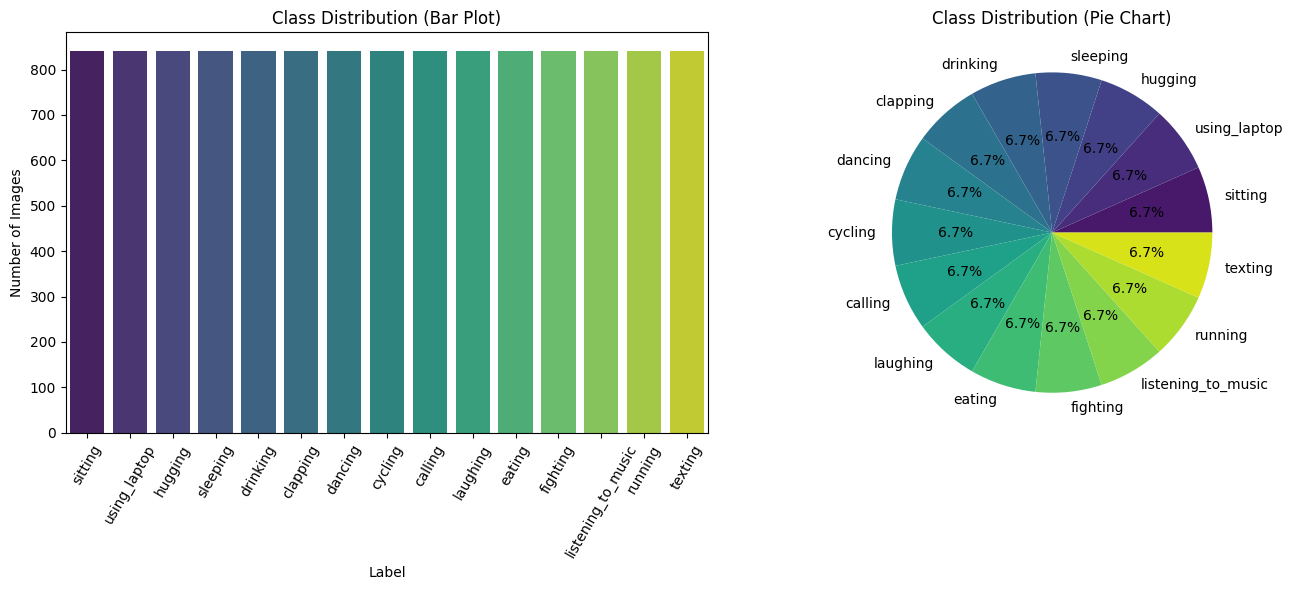
\includegraphics[scale=0.4]{assets/1b.png}
        \caption{Class Distribution of Images}{}
        \label{fig:1b}
    \end{minipage}
\end{figure}
\hspace{-3pt}
The class distribution of images is equal. But by displaying some random images of each class, I observed that some images have watermarks and text, which might affect the overall accuracy of our model

\vspace{30pt}
\subsubsection*{c) Check Class Imbalance}
\begin{figure}[H] % h = here, t = top, b = bottom, etc.
    \centering
    \begin{minipage}{0.75\linewidth}
        \centering
        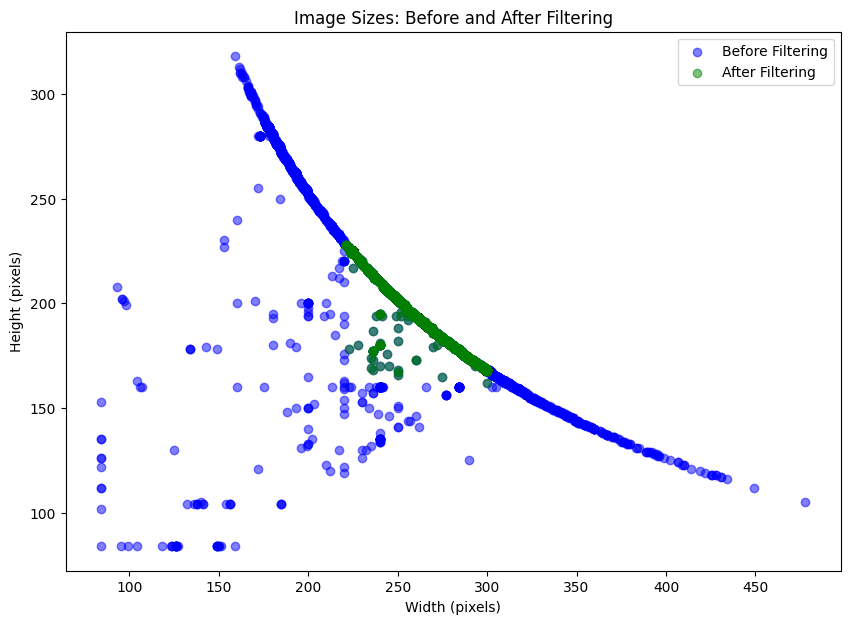
\includegraphics[scale=0.4]{assets/1c.png}
        \caption{Comparison of Image Sizes Before and After Filtering}{}
        \label{fig:1c}
    \end{minipage}
\end{figure}
\hspace{-3pt}
In the initial dataset, there is no class imbalance, but after data filtration, there might be chances of class imbalance, so we have to take care of that before feeding data to the model.

\vspace{10pt}
\subsection*{Part B: Feature Extraction}
\hspace{0pt}I extracted features using four different types of techniques:-

\begin{enumerate}
\item \textbf{Histogram of Oriented Gradients (HOG)}: For extracting texture features.
\item \textbf{Color Histograms}:- To distinguish objects in the image based on colour composition.
\item \textbf{Scale Invariant Feature Transform (SIFT)}:- To match objects in images with different viewpoints.
\item \textbf{Canny Edge Detection}:- To extract object boundaries.
\end{enumerate}
By the combination of the above four techniques, I extracted \textbf{100656} different features. After that, I split the features into training and testing sets; then, on the testing set, I first applied standardization, then PCA for Dimensionality Reduction. After that, I applied Features resampling using SMOTE, and then our features were ready to be passed in the model for training.

\vspace{10pt}
\subsection*{Part C: Model Selection and Evaluation}
\begin{figure}[H]
    \centering
    \begin{minipage}[c]{0.45\linewidth}
        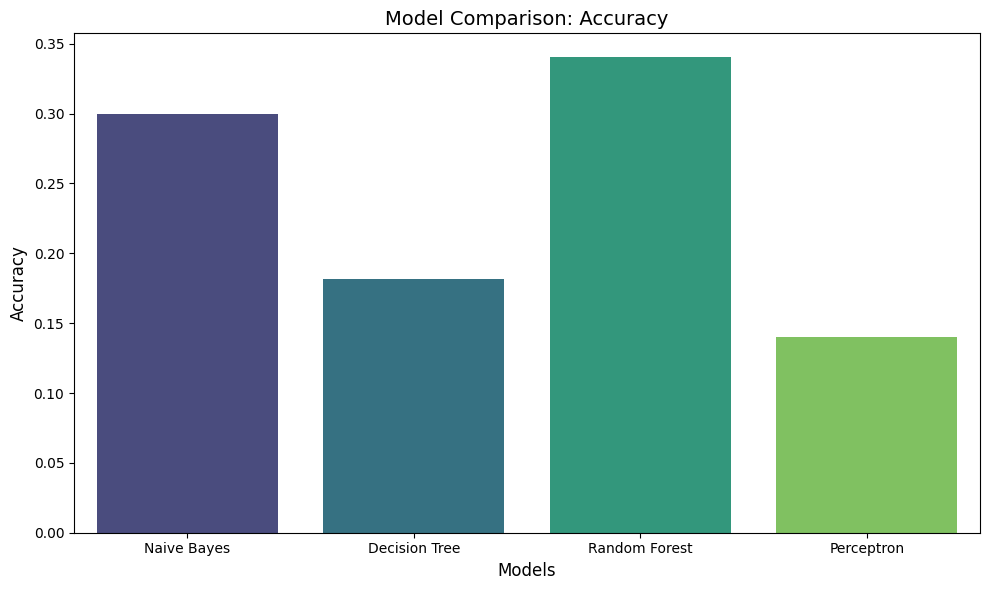
\includegraphics[scale=0.3]{assets/3.png}
        \caption{Models vs Accuracy Graph}
        \label{fig:a}
    \end{minipage}
    \begin{minipage}[c]{0.45\linewidth}
        \centering
        \vspace{0.5cm}
        \begin{tabular}{|l|c|c|}
            \hline
            Model & Accuracy \\ \hline
            Naive Bayes & 0.299376 \\ \hline
            Decision Tree & 0.181913 \\ \hline
            Random Forest & 0.351937 \\ \hline
            Perceptron & 0.139813 \\ \hline
        \end{tabular}
        \captionof{table}{Models Accuracy Table}
    \end{minipage}
\end{figure}

\hspace{-3pt}
 From the Results, I observed that Random Forest performed the best among the models due to its ensemble nature. Second is Naive Bayes, which might struggle due to highly correlated data. The decision tree and Perceptron model perform very poorly because the Decision tree will get overfitted, and the perceptron model is very simple in nature, so it can't handle the complex image data.

% \clearpage % This ensures the page break happens here

% \vspace{10pt}
% \subsection*{Solution (f)}
% \subsubsection*{Early Stopping and its Effect of Overfitting and Generalization}
% \begin{figure}[H] % h = here, t = top, b = bottom, etc.
%     \centering
%     \begin{minipage}{0.49\linewidth}
%         \centering
%         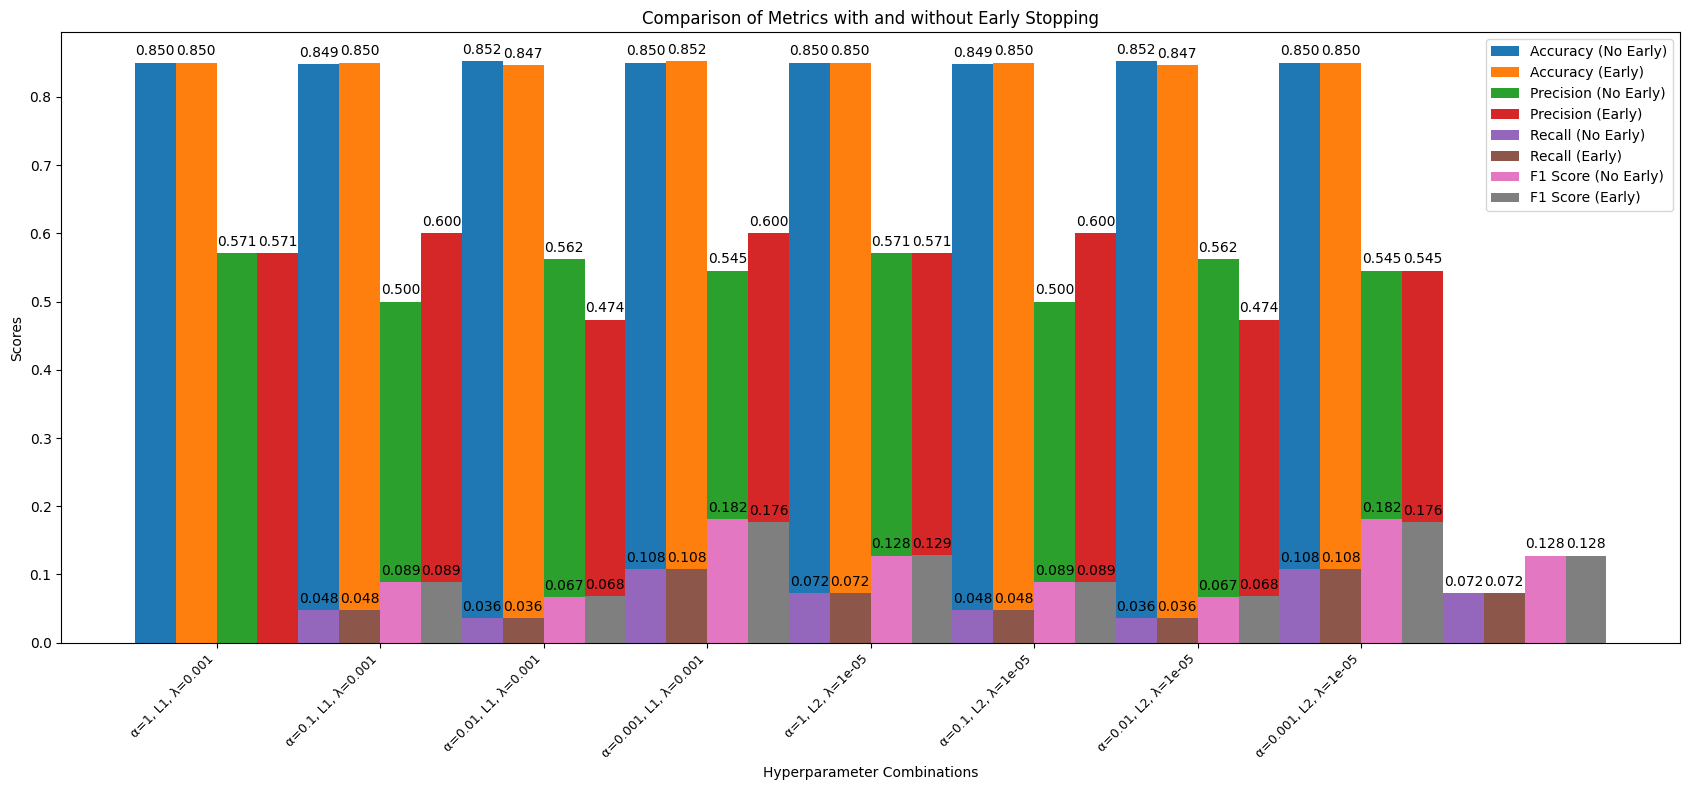
\includegraphics[width=\linewidth]{assets/fV.png}
%         \caption{Validation Dataset}{}
%         \label{fig:b-1}
%     \end{minipage}
%     \hfill
%     \begin{minipage}{0.49\linewidth}
%         \centering
%         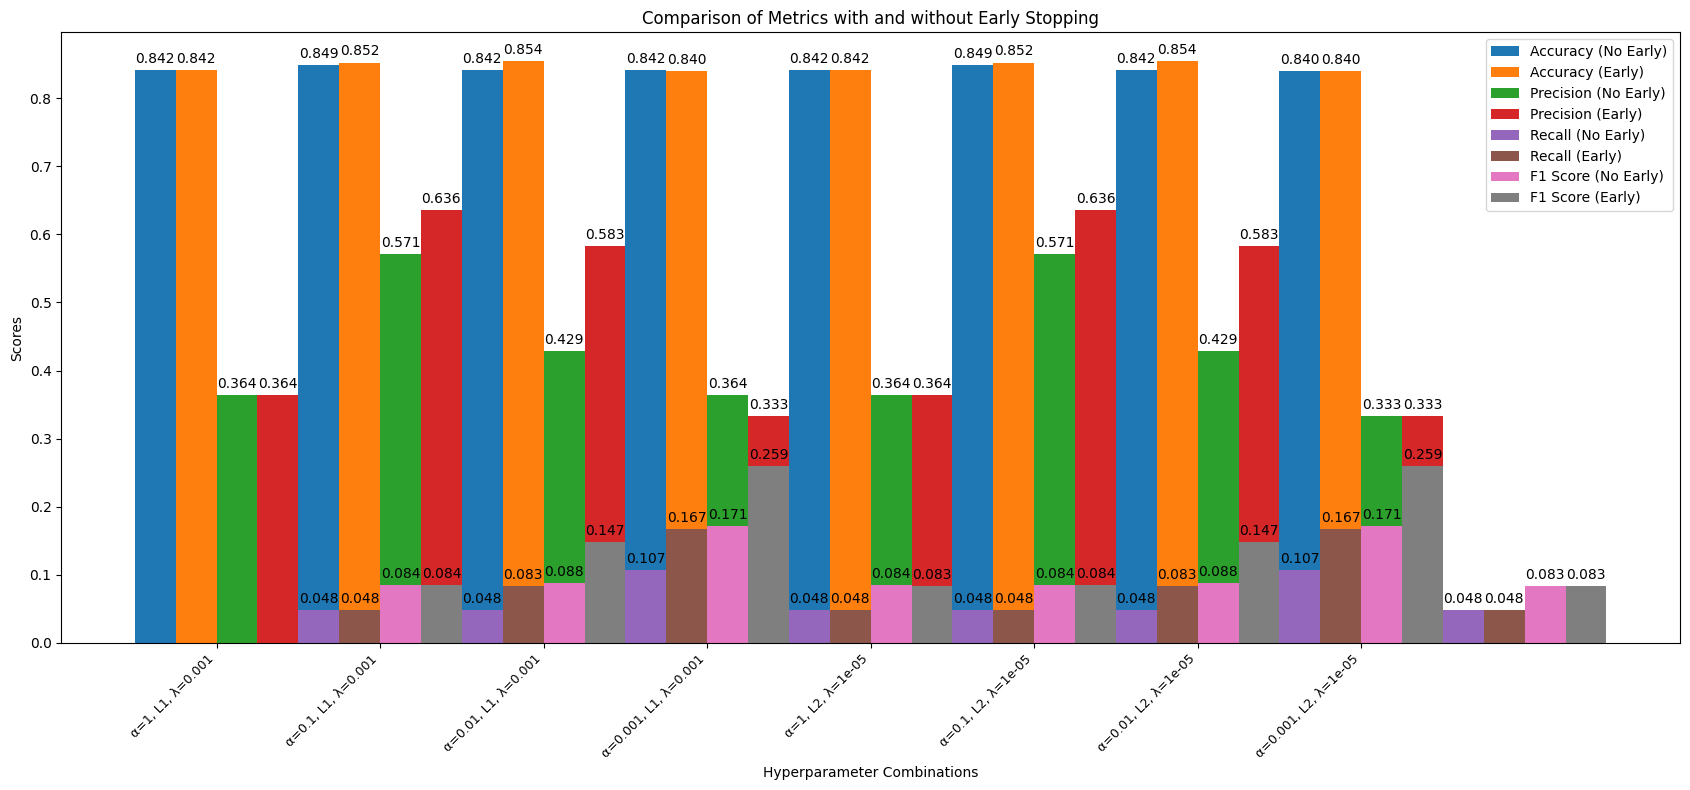
\includegraphics[width=\linewidth]{assets/fT.png}
%         \caption{Test Dataset}{}
%         \label{fig:b-2}
%     \end{minipage}
%     \caption*{Comparing impact of Early Stopping \& No Early Stopping}
% \end{figure}

% \hspace{-20pt}
% \begin{table}[H]
% \centering
% \resizebox{\textwidth}{!}{
% \begin{tabular}{|c|c|c|c|c|c|c|}
% \hline
% $\alpha$ & Regularization & $\lambda$ & Accuracy (ES/NO-ES) & Precision (ES/NO-ES) & Recall (ES/NO-ES) & F1 (ES/NO-ES) \\ 
% \hline
% 1     & L1  & 0.001  & (0.8415, 0.8415) & (0.3636, 0.3636) & (0.0476, 0.0476) & (0.0842, 0.0842) \\ \hline
% 0.1   & L1  & 0.001  & (0.8525, 0.8488) & (0.6364, 0.5714) & (0.0833, 0.0476) & (0.1474, 0.0879) \\ \hline
% 0.01  & L1  & 0.001  & (0.8543, 0.8415) & (0.5833, 0.4286) & (0.1667, 0.1071) & (0.2593, 0.1714) \\ \hline
% 0.001 & L1  & 0.001  & (0.8397, 0.8415) & (0.3333, 0.3636) & (0.0476, 0.0476) & (0.0833, 0.0842) \\ \hline
% 1     & L2  & 1e-05  & (0.8415, 0.8415) & (0.3636, 0.3636) & (0.0476, 0.0476) & (0.0842, 0.0842) \\ \hline
% 0.1   & L2  & 1e-05  & (0.8525, 0.8488) & (0.6364, 0.5714) & (0.0833, 0.0476) & (0.1474, 0.0879) \\ \hline
% 0.01  & L2  & 1e-05  & (0.8543, 0.8415) & (0.5833, 0.4286) & (0.1667, 0.1071) & (0.2593, 0.1714) \\ \hline
% 0.001 & L2  & 1e-05  & (0.8397, 0.8397) & (0.3333, 0.3333) & (0.0476, 0.0476) & (0.0833, 0.0833) \\ 
% \hline
% \end{tabular}
% }
% \caption{Comparison of Early Stopping (ES) and No Early Stopping (NO-ES).}
% \end{table}



% \hspace{-15pt}To prevent overfitting, I choose the early stopping parameter as patience = 10 and min\_delta = 1e-3. This means that training will stop if the validation loss does not improve by at least 1e-3 for 10 consecutive epochs.
% \vspace{5pt}
% \newline\hspace{-15pt}After trying eight different combinations of learning rate ($\alpha$) = \{1, 0.1, 0.01, 0.001\} and L1, L2 regularization, I come to the conclusion that early stopping stops the overfitting and promotes the generalization of the unseen test data. As it will be clearly visible in the metrics data. From all combinations of models in which early stopping is enabled, has better accuracy, precision, recall, and F1-score.

\end{document}
